\section{Variance Reduction}
\begin{frame}{}
    \LARGE Reinforcement Learning: \textbf{Variance Reduction}
\end{frame}

\begin{frame}{Variance Reduction}
\begin{itemize}
    \item However, there is a problem.
    \item This approach suffers from high variance because credit assignment is difficult.
    \item Can we help the estimator?
    \pause
    \item \textbf{First idea --- the Causality Trick:} Rewards before time $t$ cannot be affected by action $a_t$, so they carry no useful gradient signal. Use only future rewards:
    $$\nabla_\theta \mathcal{J}(\theta) \approx \sum_{t \geq 0} \left( \sum_{t' \geq t} r_{t'} \right ) \nabla_\theta \log \pi_\theta (a_t|s_t) $$
\end{itemize}
\end{frame}

\begin{frame}{Variance Reduction}
\begin{figure}
\centering
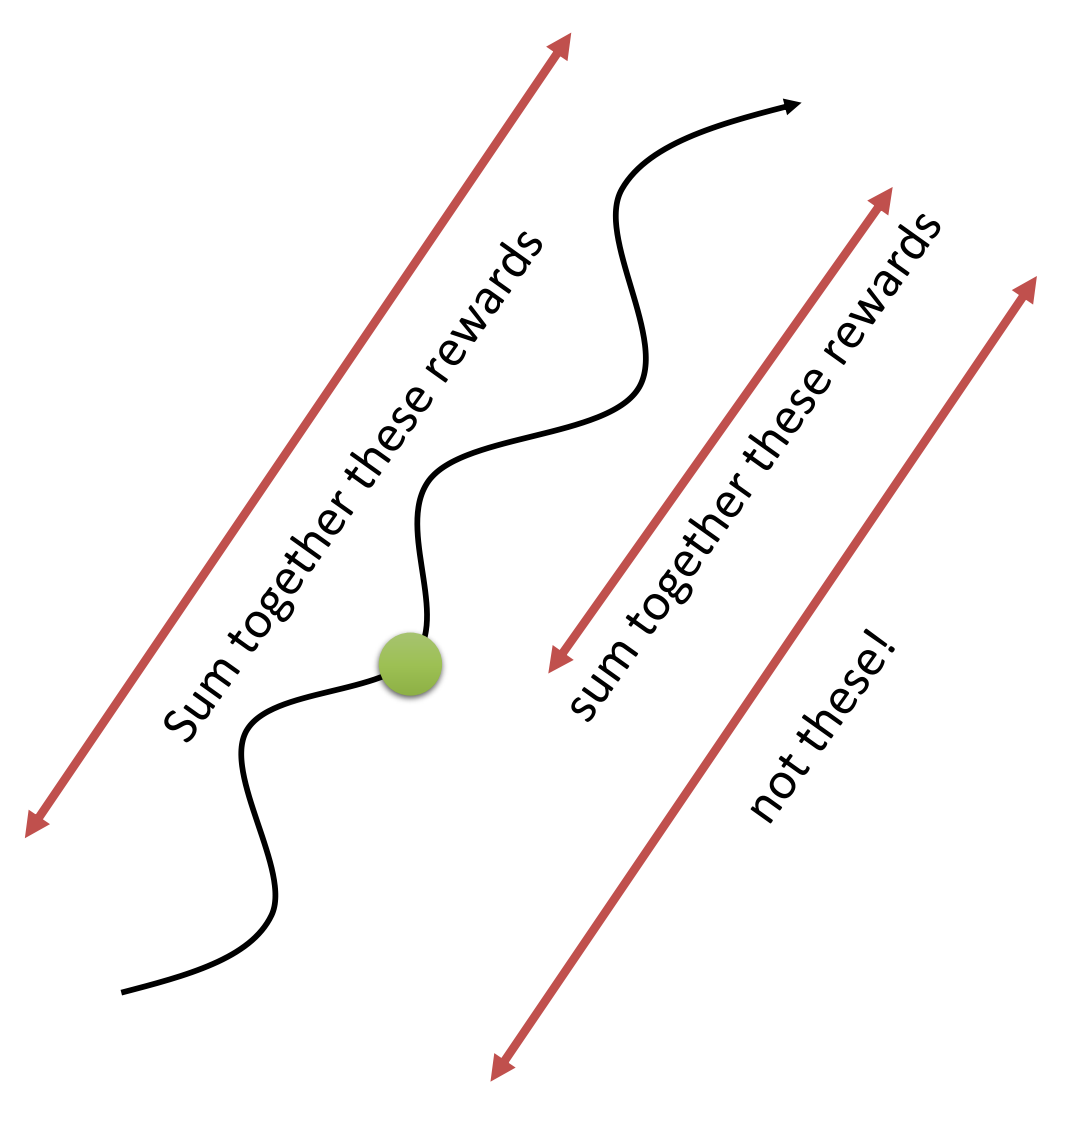
\includegraphics[width=0.9\textwidth,height=0.9\textheight,keepaspectratio]{images/vanilla-policy-gradient/var_red_1.png}
\end{figure}
\end{frame}

\begin{frame}{Variance Reduction}
\begin{itemize}
    \item The causality trick is \textbf{unbiased} --- removing past rewards is mathematically correct.
    \item But Monte Carlo returns over full trajectories are still noisy --- \textbf{high variance remains}.
    \pause
    \item \textbf{Second idea:} Weight future rewards by $\gamma^{t'-t}$, so distant rewards contribute less. This introduces a small \textbf{bias} but significantly reduces variance:
    $$\nabla_\theta \mathcal{J}(\theta) \approx \sum_{t \geq 0} \left( \sum_{t' \geq t} \gamma^{t'-t} r_{t'} \right ) \nabla_\theta \log \pi_\theta (a_t|s_t) $$
\end{itemize}
\end{frame}

\begin{frame}{Variance Reduction}
\begin{figure}
\centering
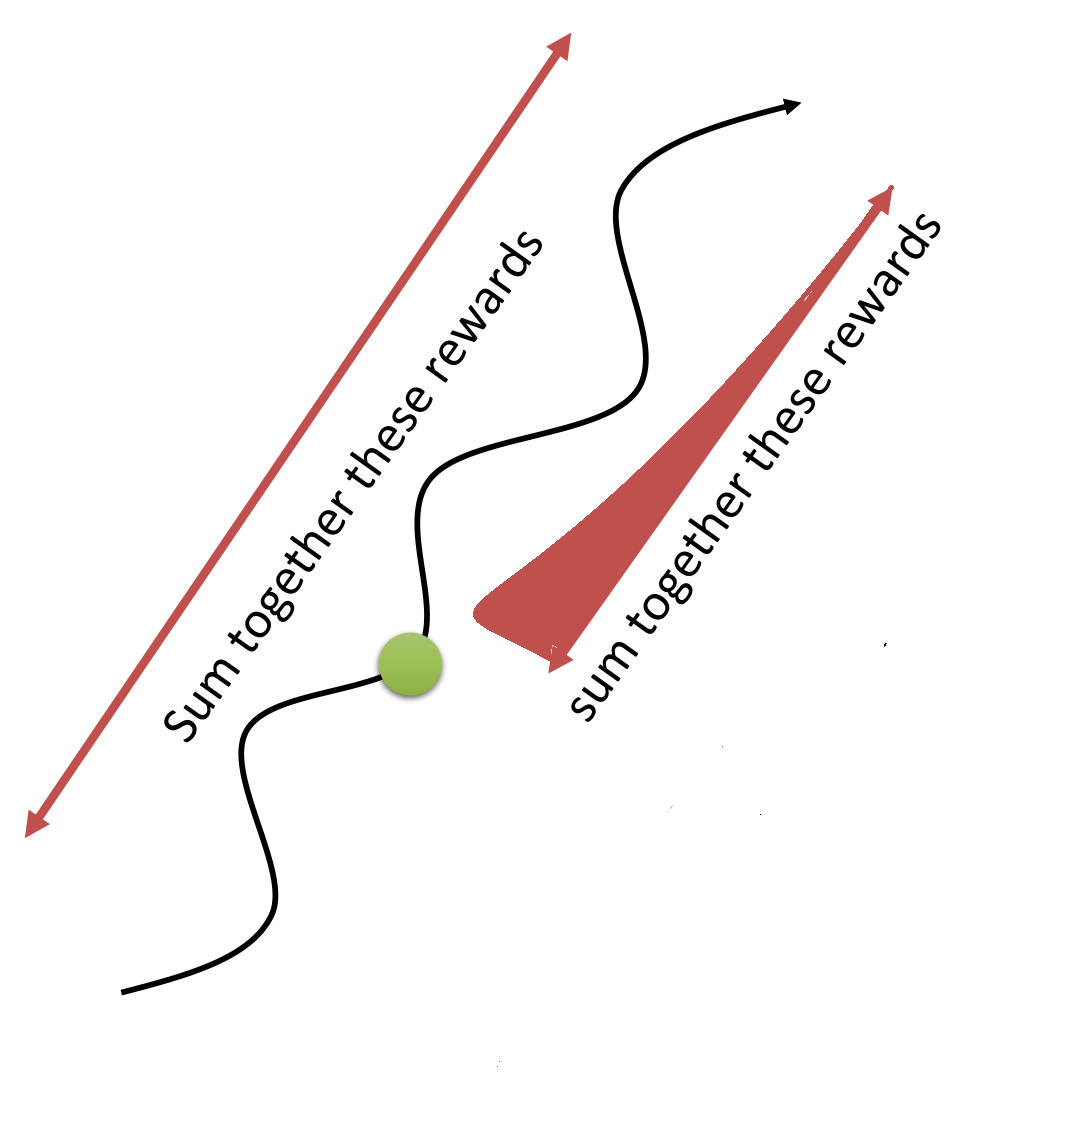
\includegraphics[width=0.9\textwidth,height=0.9\textheight,keepaspectratio]{images/vanilla-policy-gradient/var_red_2.png}
\end{figure}
\end{frame}

\begin{frame}{Variance Reduction - Baselines}
\begin{itemize}
    \item \textbf{Problem:} The raw value of a trajectory isn’t necessarily meaningful. For example, if all rewards are positive, you keep increasing the probabilities of actions.
    \pause
    \item \textbf{What is important then?} Whether a reward is better or worse than what you expect to get.
    \pause
    \item \textbf{Idea:} Introduce a baseline function dependent on the state:
    $$\nabla_\theta \mathcal{J}(\theta) \approx \sum_{t \geq 0} \left( \sum_{t' \geq t} \gamma^{t'-t} r_{t'}  - b(s_t)\right ) \nabla_\theta \log \pi_\theta (a_t|s_t) $$
    \pause
    \item A simple baseline: the moving average of rewards experienced so far from all trajectories.
\end{itemize}
\end{frame}

\begin{frame}{How to Choose the Baseline?}
\begin{itemize}
    \item Can we choose a better baseline?
    \item Essentially, we want to increase the probability of an action from a state if this action was better than the \textbf{expected value} from that state.
    \pause
    \item What does this remind you of?
    \pause
    \item \textbf{Recall from Day 1:} We defined the \textbf{Advantage function}:
    $$A^{\pi}(s,a) = Q^{\pi}(s,a) - V^{\pi}(s)$$
    \item $A^{\pi}(s_t, a_t) > 0$: action $a_t$ was better than average --- increase its probability.
    \item $A^{\pi}(s_t, a_t) < 0$: action $a_t$ was worse than average --- decrease its probability.
\end{itemize}
\end{frame}

\begin{frame}{The Advantage as a Baseline}
\begin{itemize}
    \item Using the advantage as our baseline gives us the estimator:
    $$\nabla_\theta \mathcal{J}(\theta) \approx \sum_{t \geq 0} A^{\pi}(s_t, a_t) \, \nabla_\theta \log \pi_\theta (a_t|s_t) $$
    \item This is the best possible baseline: it directly measures how much better an action was than the policy's own average.
    \item It is unbiased, and it provides lower variance than a fixed moving-average baseline.
\end{itemize}
\vspace{0.5em}
\textit{How to estimate $A^{\pi}$ in practice? We only need to learn $V_\phi$: the TD residual $r_t + \gamma V_\phi(s_{t+1}) - V_\phi(s_t)$ approximates $A^{\pi}(s_t, a_t)$, so $Q^{\pi}$ never needs to be estimated explicitly. This is covered on Day 4.}
\end{frame}
